% ABLS - term-long paper

\documentclass{sig-alternate}

\usepackage{url}
\usepackage{color}
\usepackage{enumerate}
\usepackage{balance}
\usepackage{verbatim}
\usepackage{enumitem}
\usepackage[table]{xcolor}
\usepackage{multicol,multirow}
\usepackage{subfig}
\usepackage{dcolumn}
\usepackage{palatino}
\usepackage{bbm}
\usepackage{url}
\usepackage{verbatim}
\usepackage{algorithm}
\usepackage[noend]{algorithmic}
\usepackage{fancybox, fancyvrb}
\usepackage{listings}

\permission{}
\CopyrightYear{2012}
%\crdata{0-00000-00-0/00/00}
\begin{document}

\title{ABLS - An Attribute Based Logging System for the Cloud}
\numberofauthors{1}
\author{
\alignauthor{
Christopher A. Wood \\
Department of Computer Science \\
{\tt caw4567@rit.edu}
}}
\date{\today}
\maketitle
\begin{abstract}
User-based non-repudiation is an increasingly important property of cloud-based applica-tions. It provides irrefutable evidence that ties system behavior to specific users, thus enabling strict enforcement of organizational security policies. System logs are typically used as the basis for this property. Thus, the effectiveness of system audits based on log files reduces to the problem of maintaining the integrity and confidentiality of log files. In this project, we study the problem of building secure log files. We investigate the benefits of ciphertext-policy attribute-based encryption (CP-ABE) to solve a variety of log design issues. In addition, we also present the architecture and a preliminary analysis for a proof-of-concept system that fulfills the confidentiality and integrity requirements for a secure log.
\end{abstract}

\section{Introduction}
User-based non-repudiation is a system security property that provides indisputable evidence that links
specific actions to individual users (or entities) that trigger such actions. Cryptographically speaking, non-repudiation requires that the integrity and 
origin of all data should be provable. In essence, this enables system audits to be conducted that can
identify data misuse (and thus, potential security policy violations) by comparing the sources of system events
with all entities authorized to invoke these events. Therefore, treating non-repudiation as a required system 
quality attribute in the architecture is likely to become a common trend in the commercial, 
government, and even more specifically, the health-care domain.

System audits typically use log files to determine the cause and effect of events that took 
place during the system's lifetime. In order to provide accurate information for non-repudiation purposes,
it is often necessary to place some amount user-sensitive data in these log files that can be used
to trace data back to its origin. As such, logs of events generated by a client that is being served must
maintain data confidentiality and integrity should the system be compromised. These goals are commonly achieved
using a combination of encryption and signature techniques \cite{Ma2008-FssAgg}. However, traditional approaches to
encryption and signature generation and verification are becoming less effective in the context of cloud
applications. Furthermore, naive approaches to log security that are based on tamper-resistant hardware and 
maintaining continuous secure communication channels between a log aggregator and end user are no longer useful in 
the context of cloud-based applications \cite{Schneier1999-Secure}. 

Symmetric-key and public-key encryption of log entries are very common confidentiality techniques 
proposed in the literature. However, in cloud-based applications, these schemes are becoming less useful.
There is a need for a robust access control mechanism that enables dynamic user addition and revocation
with minimal overhead (i.e. re-encrypting a subset of the log database should be avoided). Both symmetric- and 
public-key cryptosystems lack in that access policies must be tied directly to keys used for
encryption and decryption. If the access policy for a set of log messages needs to be changed, then both the keys used to
encrypt and decrypt such log entries will need to be regenerated and distributed, and the entries must also
be re-encrypted. Both of these tasks can be very expensive. 

In addition, symmetric-key cryptosystems require keys to be shared among users who need access to the 
same set of logs, which requires a secure and comprehensive key management and distribution policy. 
From a storage perspective, public-key cryptosystems (e.g. RSA and ElGamal) suffer from the extra data transfer and 
storage requirements for large cryptographic keys and certificates. There may be insufficient resources 
to maintain a public-key infrastructure (PKI) for managing keys and digital certificates for all users. 

In terms of log file integrity, aggregate signature schemes that support forward secrecy through the use of 
symmetric- and public-key cryptosystems are also becoming outdated \cite{Yavuz2009-BAF}. Symmetric-key schemes may promote
high computational efficiency for signature generation, but they do not directly support public verifiability for 
administrators and auditors. This means that robust key distribution schemes or the introduction of a trusted third party (TTP) are needed to ensure all required parties can access the necessary log information. Such schemes also 
suffer from high storage requirements and communication overhead. Public-key schemes have similar issues, 
as the increased key size leads to even larger storage requirements and less computational efficiency. 

Collectively, we see that a balance between encryption and signature generation and verification performance is
needed to support the unique scalability and resource usage requirements for cloud-based applications.
Attribute-based encryption (ABE), a new cryptographic scheme that uses user attributes (or roles, in certain 
circumstances) to maintain the confidentiality of user-sensitive data, has an appealing application
to logging systems maintained in the cloud and is capable of satisfying the aforementioned confidentiality 
requirements. In addition, authenticated hash-chains have been shown to be effective at enforcing log file integrity
in numerous logging schemes  \cite{Schneier1999-Secure}. 

ABLS, an attribute-based logging system that supports 
ciphertext-policy attribute-based encryption (CP-ABE) 
\cite{Bethencourt2007-CPABE} and authenticated hash-chain constructions for log file confidentiality and integrity, 
respectively, is a logging system designed for the cloud to address the aforementioned problems. This paper
describes the motivation and design of ABLS, as well as some implementation details of the prototype. The paper
concludes with a discussion of the current status of the project and planned work to be completed.

\section{Prototype Implementation}
In order to test both the correctness and performance of ABLS, a proof-of-concept system has been
developed. In this section we provide the design and rationale for the prototype architecture.

\subsection{Deployment}
\label{sec:deployment}
ABLS is designed to be a centralized logging system backed by a set of distributed databases. A context
diagram for the ABLS deployment scheme is shown in Figure \ref{fig:deployment}.

%TODO: rough deployment diagram for ABLS (different from architecture diagram)

\begin{figure*}[htb!]
\label{fig:deployment}
\begin{center}
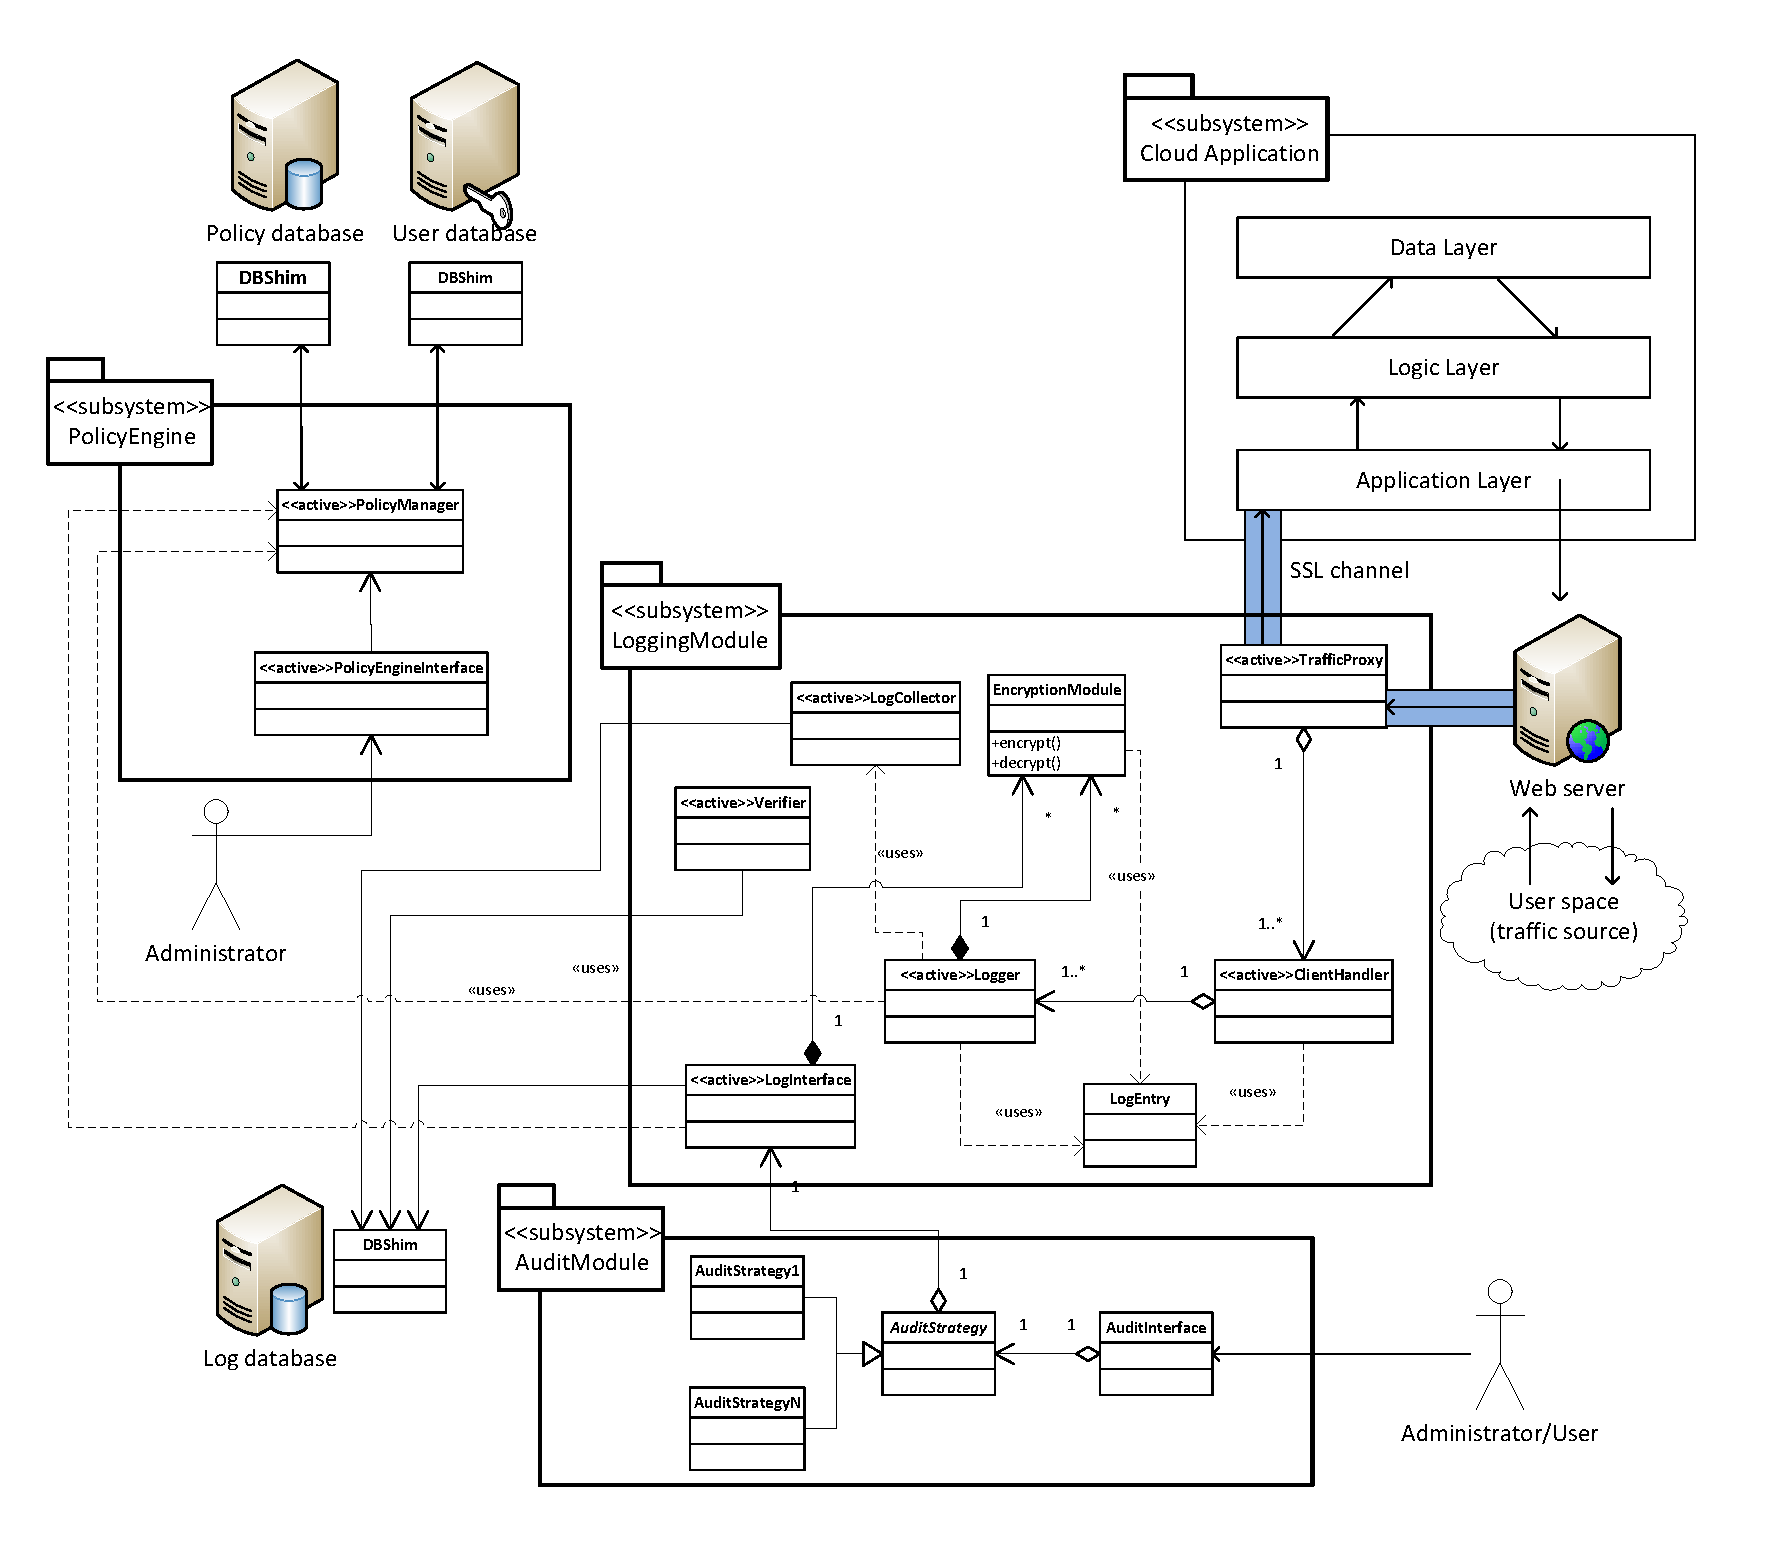
\includegraphics[width=7in]{images/design.pdf}
\caption{The deployment strategy and a detailed design for ABLS.}
\end{center}
\end{figure*}

Based on the purpose of each piece of database used in the log, it is best to physically separate databases
that store data of different security classes rather than rely on MAC with polyinstantiation. Of course, access control
and authentication mechanisms for all database servers is enforced at the operating system level, thus
prohibiting immediate access to all unauthorized users other than the {\tt LoggingModule} and {\tt PolicyEngine} 
processes. 

In the current ABLS prototype, all database servers are separated as individual SQLite database files. Once
the deployment platform is selected and properly configured, these will be replaced with instances of MySQL 
databases running on separate servers.

\subsection{Hybrid Key Management}
\label{sec:keyMgmt}
In order to increase the performance of log entry encryption during a given user session, symmetric-key encryption
using AES-256 is chosen to encrypt all log entry messages. The symmetric key is then encrypted using the CP-ABE
scheme. This design enhancement enables increased improvement without sacrificing the level of confidentiality 
granularity that is needed for each log entry. 

The basic algorithm for encrypting a log entry is shown in Algorithm \ref{alg:encrypt}. Once encrypted, the cipher text
is stored as specified in Section \ref{sec:LogConstruction}.

\begin{algorithm}[ht!] %[htb]
\caption{Log entry encryption} \label{alg:encrypt}
\begin{algorithmic}[1]
\REQUIRE{An unencrypted log entry $L_i$ for session $S_j$ of user $U_k$}
% \ENSURE{The number of all minimum $(s,t)$-cuts of $G$}

% I decided not to list the input/output in this case, so that's why the above two lines are commented out
\STATE{Let $P$ be the access control policy for the message of $L_i$, as determined by the {\tt PolicyManager}}
\IF{The symmetric key $K$ for $(U_k, S_j)$ has not been generated for $P$}
	\STATE{Generate $K$ and encrypt it (with the CP-ABE encryption module) using $P$}
	\STATE{Persist $K$ to the key database}
\ENDIF
\STATE{Encrypt $L_i$ with AES-256 using $K$, yielding $E(L_i, K)$}
\STATE{Persist $(L_i, K)$ to the log database}
\end{algorithmic}
\end{algorithm}

\subsection{Database Design}
\label{sec:databaseDesign}
As shown in section \ref{sec:deployment}, there are four main databases that must be maintained by ABLS:
the log, key, user, and policy database. The log database maintains the all information in the log chain for every 
single user and session pair. The key database stores the cryptographic keys that were used to construct
such log chains. The user and policy databases store user information and policy rules for ABLS, respectively. 
In the current prototype of ABLS, the policy database is not used externally. All event rules are hard-coded into
the {\tt PolicyEngine}. 

In order to link the entries in the log tables to their corresponding verification and encryption keys in the key database,
common user and session IDs are used (though not as the primary key for the tables since they do not satisfy
the uniqueness property). However, because such the storage of such user and session information in plaintext
may lead to violation of user privacy, they are deterministically masked before being stored in the database. This technique
was inspired by CryptDB \cite{Popa2012-CryptDB}.

This masking procedure works by encrypting the user and session attributes with a symmetric key generated
by the logger's master key salted by the user's unique identifier. Specifically, the encrypted user and session IDs, $[U_i]$ 
and $[S_j]$, stored in table T are generated as follows.
\begin{align*}
[U_i] = E(M_k || H(U_i) || H(T), U_i) \\
[S_j] = E(M_k || H(U_i) || H(T), S_j) \\
\end{align*}

In this context, $M_k$ is the master key for the logger. Using the user and table identifiers as salts to the master key 
enable ensures that tables do not share any common information about the user, which helps prevent against 
inference attacks.

\section{Completed Work}
For Phase 1 of the project, I focused mainly on fixing some of the design and implementation flaws in my previous 
prototype, redesigning the database to support the new symmetric key management scheme and data 
partitioning for different security classes, specifying the deployment scheme, and improving the quality test
of my internal unit tests and the functionality of the test driver program. The specifics of each of these improvements is
outlined in the following sections.

\subsection{Hybrid Key Management}
As described in Section \ref{sec:keyMgmt}, the process of encryption log messages was changed to use symmetric-key
encryption instead of CP-ABE due to the added performance improvement. Pairing-based cryptography is computationally
expensive, and under the assumption that ABLS might be subject to very heavy traffic loads at any particular time, the 
overhead of encrypting data to be stored in the database should be as minimal as possible. Therefore, each unique
policy that is needed to encrypt a log message is associated with a symmetric key, which is in turn encrypted and 
serialized using CP-ABE. The Charm crypto package allows all cryptographic objects (which tend to be nested
Python dictionaries and other complicated data structures) to be serialized to byte representations for database 
persistence. 

Also, in order to improve the performance of the logger, the per-policy symmetric keys for a user session are kept
in memory until the session has been closed. This avoids the need for the logger to query the database for the key 
when a new piece of data to be inserted into the log. 

Unfortunately, with this new key management scheme, the verification procedure becomes dependent on the
logger's master key. Thus, I have to implement a mechanism to share this key between the two entities. I expect
to complete this modification for Phase 2 of the project.

\subsection{Relational Database Design}
The relational database design was modified in order to support the new symmetric key management scheme and provide 
enhanced security for the stored data. In particular, rather than storing the cryptographic keys in the same database as the
log information, these two databases are now segregated and are expected to be deployed on different database servers.
By hardening both databases, a malicious attacker would need to circumvent the access control mechanisms protecting
two physically disjoint databases, rather than just one. 

In addition, to better support audits that use the log database, a timestamp field was added to each table as a required
attribute. Not only does such information capture the exact timing of critical system events, it acts as a protection
mechanism in the event that log messages are inserted into the database out of order. Also, it is important to note that
each and every timestamp for a log message is generated as soon as the {\tt ClientHandler} reads the data from
its open socket. This is done to provide the most accurate timing information.

%Redesigned the relational database model to account for the different security classes among data that is used by ABLS. This resulted in a physical separation of database servers.
%TODO: added times, separated the database tables, optimized data types for columns to match what's stored

\subsection{Database Column Masking}
The initial implementation of the database masking procedure, which is outlined in Section \ref{sec:databaseDesign}
was started in this phase of the project. Currently, only the ability for the logger to store the encrypted user and session IDs 
is supported. The verifiers have yet to be updated to use this encrypted data to perform the strong verification check. This 
will finished in the next phase of the project.

\subsection{Bootstrapping, Test Enhancement, and Deployment}
In order to streamline the test and deployment phases of development, a bootstrap script was implemented to configure
new (empty) versions of the local SQLite databases. The main executable script (main.py) was also modified to support
debug and production modes of operation, in which the debug mode clears the contents of every database and
then proceeds to insert false user data into the users table to begin the logging process. The test driver program,
TrafficProxyDriver.py, is then modified accordingly to use the default data contained within the database. With these
changes, the typical process to start and interact with the ABLS system is as follows.

\begin{enumerate}
	\item Run the bootstrap script to create new versions of the local SQLite databases. In the actual deployment of an ABLS system, this script would connect to the remote databases and re-specify their schemas accordingly. Thus, it is meant only for development purposes and should not be used on a live ABLS instance.
	\item Run the main executable file (main.py) with the -c (clear) to flag to enable debug mode, in which the databases are wiped clean and replaced with a small set of fake data. If you wish to start the ABLS system at this point in time, you may also add the -s (start) flag to the script so that it starts the ABLS instance.
	\item Run the test driver program (TrafficProxyDriver.py) and point it to the host and port at which the traffic proxy within the ABLS instance is listening. By default, this is ``localhost'' and port 9998, but this can easily be configured in the source code. 
\end{enumerate}

Aside for the initialization code, the test driver program now includes a more robust suite of tests to simulate varying traffic 
loads. The user interface of this program was also improved so as to aid the developers in interacting with the ABLS 
prototype at runtime. Given the difficulty of testing this distributed system at runtime, creating a more sophisticated
test driver was crucial to the development process that enabled smoke tests to be run with minimal effort.

However, despite the increased complexity of the test driver, it does not, nor will it ever, support the ability to acquire 
diagnostic information from the ABLS runtime. This information is logged by the ABLS runtime to the appropriate log 
file, and the administrators for the ABLS system can check this information at their discretion.

%The system deployment strategy was finalized 

\subsection{Outstanding Bug Fixes}
As a result of resuming my work from the previous quarter, some of my time spent during Phase 1 was devoted to fixing
outstanding design and performance bugs in the ABLS prototype. Some of the notable bugs include improper 
initialization of the verifier threads and incorrect management of the in-memory data structures containing the 
user session information (i.e. data specific to the generation of log messages).

\subsection{Research and Literature Survey}
An initial action item for this work was to investigate the possibility of replacing the relational database model with a 
NoSQL model. I spent a significant amount of time during week 4 investigating the benefits of making a transition
to such a DBMS. In particular, I examined MongoDB, a common document-based NoSQL database. Unfortunately,
my research revealed that MongoDB is not an ACID system, and thus transactions are not guaranteed to keep the
database in a consistent state. In the context of ABLS, a failed transaction could put the system in a bad state. Therefore,
I made the decision to keep the relational database model but hide the user-sensitive information using the techniques
discussed in Section \ref{sec:databaseDesign}.

A comprehensive literature survey on related logging and non-repudiation work was also completed during this phase 
of the project. The corresponding articles that were read are included in this phase's submission package. The digest of this work is expected to be a part of the final report and potential publication.

\subsection{Log Traffic Encryption}
TODO

\section{Future Work}
For the remainder of the project I plan to finish up the partially completed work introduced in the previous section and 
focus on the auditing aspect of ABLS. Auditing will be supported both manually and automatically through
a robust log query interface, which places the ABLS runtime in the role of the reference monitor, and automated
strategy-driven tasks run within the context of the ABLS runtime, respectively. The following sections expand upon all
of these action items in more detail.

\subsection{Log Collection - 1/12/13}
As part of the proposed design, all log messages generated by the logger to be inserted into the 
database will be handed off to a common log collector to do so. This log collector will be implemented as a 
separate actor (thread) running within the ABLS process and will assume a portion of the database 
communication overhead from the logger to free up cycles for processing more log messages. 

\subsection{Complete Database Masking - 1/15/13}
Following the design outlined in Section \ref{sec:databaseDesign}, the database masking scheme will be completed by
adding support to the database verifiers. Since the verifiers run within the context of the ABLS system, they will be granted
permission to all of the database servers so that they may request the appropriate entity and epoch keys used to perform
strong verification checks on the data in user session log chains. Also, this must be the first activity that is completed 
because the log querying and automated audit tasks depend on the database columns being properly masked. 

\subsection{Log Querying - 1/19/13}
In order to make ABLS fulfill its purpose as a secure logging system, log query support will be added to the audit
module. Such query support will be exposed to clients through a lightweight API that is used via the auditing protocol.
To start, only select operations will be supported, and they can be parameterized by the user ID or both the user and 
session IDs. As an example, the API might have the following function signatures. \\

\noindent {\tt selectByUser(int uid)} \\
{\tt selectByUserAndSession(int uid, int sid)}\\

Clients will connect to an audit proxy, which is similar to the log traffic proxy, and issue commands according to
the audit protocol to invoke either one of these functions. Client authentication is expected to be completed at a later
point in time as outlined in Section \ref{sec:auth}. Assuming the client has been authenticated, they can issue commands
wrapped in JSON strings to the audit proxy that have the following format. \\

\begin{lstlisting}
{     
    "command" : command_id
    "params" : csv_list
}
\end{lstlisting}

Upon receiving and parsing an incoming command, the audit proxy will issue the appropriate command to the log module
to select the appropriate log message contents from the database. However, since each client is expected to be a user for
ABLS, their attributes will be used to filter the resulting database rows that are returned. Thus, the audit proxy will act
as a reference monitor that enforces access control to the log database through the log query protocol and API.

In order to implement this task, I will perform the following steps.

\begin{enumerate}
	\item Implement the audit proxy with a corresponding client handler thread using the same technique that was done for the traffic proxy. 
	\item Implement the functionality in the client handlers to parse messages according to the log query protocol.
	\item Implement the functionality to collate log message for the specific client in a temporary location.
	\item Using the client's attributes, filter all messages that cannot be decrypted according to the embedded policy.
	\item Format the results in a JSON string that is sent back to the client.
\end{enumerate}

Unlike the traffic proxy, it is expected that the clients for the audit proxy will be authenticated using passwords. Thus, as
part of supporting client authentication, a proper password storage scheme will need to be implemented, which includes 
the modification of the user database schema and the proper password hashing (and salting) techniques. 

\subsection{Audit Strategy Design - 1/24/13}
As the number of contents in the log database grows, manual audits become less appealing. Therefore, the audit module
will be extended with strategy-driven audit tasks that can scan the log database on-demand to check for policy violations.

TODO: finish

- auditing design and implementation (define automated worker tasks that use pre-defined strategies for
auditing (search by userID) or whatnot that can be triggered by any web application set in front of ABLS - 
making it easy for auditors to start their own automated audits). 

\subsection{ABLS Configuration File - 1/25/13} 
In order to improve the quality of the ABLS prototype, all of the hard-coded configuration strings that set up databases,
specify cryptographic certificate locations, log file output directories, etc will be removed and placed in a configuration file
to be managed by system administrators. Access to this file will be restricted to system administrators and enforced by the 
operating system. An example of how the configuration file might look is shown below.

\begin{lstlisting}
# comment
log_database: network location string
key_database: network location string
user_database: network location string
log_file: absolute path string
...
\end{lstlisting}

\subsection{Client Authentication - 1/31/13}
\label{sec:auth}

TODO: public-key authentication using SSL certificates (prefered), user logins for audit interface

\begin{comment}
\begin{table}
\centering
\caption{Feelings about Issues}
\begin{tabular}{|l|r|l|} \hline
Flavor&Percentage&Comments\\ \hline
Issue 1 &  10\% & Loved it a lot\\ \hline
Issue 2 &  20\% & Disliked it immensely\\ \hline
Issue 3 &  30\% & Didn't care one bit\\ \hline
Issue 4 &  40\% & Duh?\\ \hline
\end{tabular}
\end{table}

\begin{figure}[htb]
\label{sample graphic}
\begin{center}
\includegraphics[width=1.5in]{fly.jpg}
\caption{A sample black \& white graphic (JPG).}
\end{center}
\end{figure}
\end{comment}

\bibliographystyle{abbrv}
\bibliography{../abls}
% You must have a proper ".bib" file
%  and remember to run:
% latex bibtex latex latex
% to resolve all references
\balance
\end{document}
